\documentclass[tikz,11pt]{standalone}
\usepackage{newtxtext,newtxmath}
\usepackage{xifthen}
\usepackage{xcolor}

\usetikzlibrary{calc,positioning}

% Define sizes and parameters in cm
\def\width{10}
\def\height{6}
\def\levelsep{1.3}
\def\levelwidth{1.5}
\def\det{0.2}
\def\lrsep{3.5}

% Colors
\colorlet{darkGreen}{green!40!black!60}

% Settings
\tikzstyle{every node}        = [inner sep=0pt,outer sep=0pt]
\tikzstyle{level}             = [very thick]
\tikzstyle{axis}              = [-latex,thick]
\tikzstyle{axis label}        = [midway,left=1ex,label={[rotate=90]:#1}]
\tikzstyle{ket}               = [midway,below=2pt]
\tikzstyle{coherent coupling} = [-latex,shorten <=2pt,shorten >=2pt,thick,densely dotted,black!50]
\tikzstyle{JC doublet}        = [draw,fill,darkGreen,ultra thick,
                                 minimum width=\levelwidth cm]
\tikzstyle{JC label}          = [darkGreen,fill=white]
\tikzstyle{energy sep}        = [<->,>=latex,shorten <=1pt,shorten >=1pt,
                                 thin,densely dotted,gray]

\begin{document}
    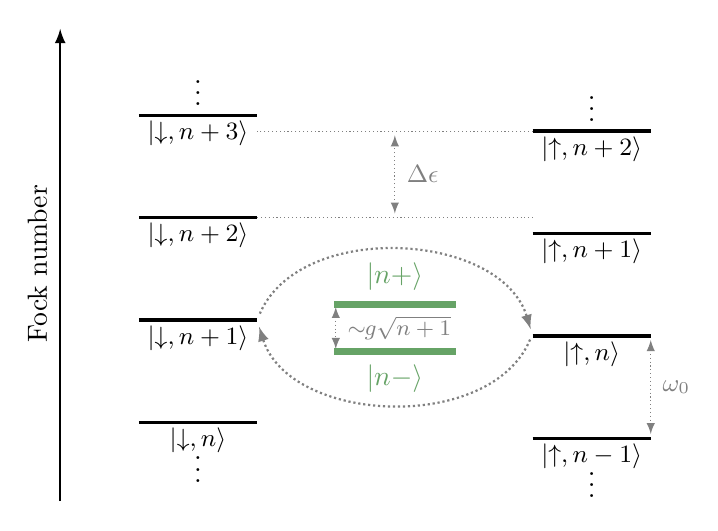
\begin{tikzpicture}
        \draw[axis] (0,0) -- (0,\height) node[axis label=Fock number] {};

        \begin{scope}[shift={(1,1)}]
            \foreach \n in {0,...,3}
            {
                \draw[level] (0,{\n*\levelsep}) --++(\levelwidth,0)
                    node[at end] (e\n) {}
                    node[ket]    (l\n) {\small $\left|\downarrow, n \ifthenelse{0 = \n}{}{+\n}\right\rangle$};
            }
            \node[below]     at (l0) {\vdots};
            \node[above=1em] at (l3) {\vdots};
        \end{scope}

        \begin{scope}[shift={($(e0)+(\lrsep,-\det)$)}]
            \foreach \n in {-1,...,2}
            {
                \draw[level] (0,{(\n+1)*\levelsep}) --++(\levelwidth,0)
                    node[at start] (w\n)  {}
                    node[ket]      (r\n)  {\small $\left|\uparrow, n \ifthenelse{0 = \n}{}{\ifthenelse{-1 = \n}{-1}{+\n}}\right\rangle$}
                    node[at end]   (er\n) {};
            }
            \node[below] at (r-1) {\vdots};
            \node[above=1em] at (r2) {\vdots};
        \end{scope}

        % JC doublet
        \node[at={($(e1)!0.5!(w0)$)},inner sep=2ex] (g) {};
        \draw[coherent coupling] (e1) to[bend left=70] (w0) edge[bend left=70] (e1);
        \node[JC doublet,label={[JC label,yshift= 1ex]above:$|n+\rangle$}] (n+) at (g.north) {};
        \node[JC doublet,label={[JC label,yshift=-1ex]below:$|n-\rangle$}] (n-) at (g.south) {};

        % Energy separations
        \draw[thin,gray,densely dotted] (e2.center) --++ (\lrsep,0)  node[midway] (du) {};
        \draw[thin,gray,densely dotted] (w2.center) --++ (-\lrsep,0) node[midway] (dd) {};

        \draw[energy sep] (du)      -- (dd)      node[midway,right=1ex] {\small $\Delta\epsilon$};
        \draw[energy sep] (er0)     -- (er-1)    node[midway,right=1ex] {\small $\omega_0$};
        \draw[energy sep] (n+.west) -- (n-.west) node[midway,right=1ex] {\footnotesize $\sim\!\!g\sqrt{n+1}$};
    \end{tikzpicture}
\end{document}

